\documentclass[aps,prd,onecolumn,11pt,nofootinbib,notitlepage]{revtex4-2}
\usepackage[T1]{fontenc}
\usepackage[utf8]{inputenc}
\usepackage{amsmath,amssymb,bm,graphicx,booktabs}
\usepackage[colorlinks=true,linkcolor=blue,urlcolor=blue]{hyperref}
\setlength{\emergencystretch}{4em}
\begin{document}
\title{Finite CMB compensation budgets in a bounded nine-moment foreground class}
\author{Anonymous methods and results note}
\noaffiliation
\begin{abstract}
Seven retained passband responses give a full-row-rank matrix for nine signed, second-order synchrotron and dust moments in each of six fixed response conventions. In the unrestricted linear class, the CMB response can consequently be represented by foreground moments in every one of the 24 signed $E_2/E_3/B_2/B_3$ coordinates. A declared joint quadratic bound changes that statement quantitatively: the least moment budget for a unit CMB response is $3.117720$--$3.118388$ target-amplitude units in one common column-normalized metric. A single foreground can compensate a target tensor displacement of norm at most $\rho/\ell_M$, while two bounded foregrounds can make two targets separated by as much as $2\rho/\ell_M$ agree on the same synthetic data. For arbitrary specified frequency data, the complete 24-dimensional compatible target set is a calculable ball or is empty. The raw-coordinate identity metric changes the unit cost to $59.572829$--$59.592192$, displaying explicit metric sensitivity. These are finite algebraic results for the declared free signed-moment class. No sky tensor, physical moment bound, joint noise law, or native solver output is used.
\end{abstract}
\maketitle

\section{Physical mechanism and frozen finite response}

A passband integrates spectral components before their angular coefficients are estimated. Spectral changes in a component's index or temperature therefore add frequency response columns to its leading spectrum. If enough independently variable moment maps are admitted, their channel responses can reproduce the CMB's calibrated response. A bound on their joint amplitude restores a finite compensation cost, even when the unrestricted response matrix spans all channels. That cost depends on which moment amplitudes the bound regards as comparable.

This note consumes the already computed, released-bandpass finite matrices in the retained R31 result identified in the accompanying claim-to-source map; it performs no passband integration or map analysis. The seven frequency rows, in order, are 030, 044, 070, 100, 143, 217, and 353PSB. The nine columns are
\begin{equation}
 (s,s_\beta,d,d_\beta,d_t,s_{\beta\beta},d_{\beta\beta},d_{\beta t},d_{tt}).
 \label{eq:order}
\end{equation}
Here $t=(T-20\,\mathrm K)/(20\,\mathrm K)$; the retained pivots are $\beta_s=-3$ in Rayleigh--Jeans temperature, $\beta_d=1.5$, $\nu_s=30\,\mathrm{GHz}$, $\nu_d=353\,\mathrm{GHz}$, and $T_{\rm CMB}=2.7255\,\mathrm K$. Taylor factorials are absorbed into the signed moment coefficients. In particular, the second temperature response uses $T_d^2\partial_T^2$, with $T_d=20\,\mathrm K$. The two LFI frequency conventions A/B and three HFI transmission thresholds $10^{-7},10^{-8},10^{-6}$ are retained as six separate finite response models. Their envelope is not a calibrated passband uncertainty.

The full target carrier has $5+7+5+7=24$ real coordinates: $E_2,E_3,B_2,B_3$, with $m=0$ followed for each positive $m$ by $(\sqrt2\operatorname{Re},-\sqrt2\operatorname{Im})$. Write the frequency-major data $Y\in\mathbb R^{7\times24}$, target $s\in\mathbb R^{24}$ and moment array $U\in\mathbb R^{9\times24}$ as
\begin{equation}
 Y=a s^{\mathsf T}+FU,\qquad a=(1,\ldots,1)^{\mathsf T}\in\mathbb R^7,
 \qquad \operatorname{vec}_{\rm row}(Y)=(a\otimes I_{24})s+(F\otimes I_{24})\operatorname{vec}_{\rm row}(U).
 \label{eq:model}
\end{equation}
All coordinates, including derivative moments, are free and signed. $s$, $U$, and $Y$ use the same target harmonic-amplitude unit, taken here as $\mu\mathrm K_{\rm CMB}$ when a unit is needed. $F$ and the metric scales below are dimensionless under the retained response normalization. There is no observed $Y$ in this experiment.

The primary class uses a single metric across all six branches:
\begin{align}
 d={}&(1.261652382369369,\;0.1777139521270542,\;1.1309894216176297,\nonumber\\
 &0.09451923139372441,\;0.04109240642871376,\;0.1151042544103929,\nonumber\\
 &0.07145402059880916,\;0.022520789584731377,\;0.09386151314750793),\nonumber\\
 M={}&\operatorname{diag}(d_1^2,\ldots,d_9^2),\qquad
 \|U\|_M^2:=\operatorname{tr}(U^{\mathsf T}MU)\le\rho^2.
 \label{eq:metric}
\end{align}
The $d_i$ are the stored column norms of the nominal A, $10^{-7}$ matrix. Thus $\rho$ is a jointly applied computational moment budget in the target-amplitude unit, not a measured foreground prior. We also compute $M=I_9$ as an explicitly different metric. Neither metric imposes physical positivity or cross-moment coupling.

\section{Minimum compensator and singular directions}

For a full-row-rank $F$ and any symmetric positive-definite $M$, define
\begin{equation}
 K=FM^{-1}F^{\mathsf T},\qquad
 c_M=M^{-1}F^{\mathsf T}K^{-1}a,\qquad
 \ell_M^2=a^{\mathsf T}K^{-1}a.
 \label{eq:min}
\end{equation}
The $7\times7$ matrix $K$ is positive definite. Lagrange multipliers for $\min_{Fc=a}c^{\mathsf T}Mc$ give $Mc=F^{\mathsf T}\lambda$, $K\lambda=a$, hence Eq.~\eqref{eq:min}. If $Fc=a$, then $c=c_M+n$ with $Fn=0$, and
\begin{equation}
 c^{\mathsf T}Mc=\ell_M^2+n^{\mathsf T}Mn.
 \label{eq:orth}
\end{equation}
This proves the unique minimum and retains the two-dimensional coefficient nullspace. It also proves that the signed compensation $\Delta U=-c_M v^{\mathsf T}$ has minimum budget $\ell_M\|v\|_2$ for any complete target displacement $v\in\mathbb R^{24}$.
For $M=\operatorname{diag}(d^2)$, let $G=F\operatorname{diag}(d)^{-1}$ and let the columns of $N_z$ span $\ker G$. The exported original moment-coordinate directions are $N_c=\operatorname{diag}(d)^{-1}N_z$, so $FN_c=0$, $N_c^{\mathsf T}MN_c=I_2$, and $N_c^{\mathsf T}Mc_M=0$. The result retains $N_z$ separately with an explicit whitened-coordinate label.

To display which response directions incur the cost, factor
\begin{equation}
 FM^{-1/2}=U_f\operatorname{diag}(\sigma_1,\ldots,\sigma_7)V_f^{\mathsf T},
 \qquad
 \ell_M^2=\sum_{i=1}^{7}\frac{(u_i^{\mathsf T}a)^2}{\sigma_i^2}.
 \label{eq:svd}
\end{equation}
The first seven rows of $V_f^{\mathsf T}$ are orthonormal directions in whitened coefficient coordinates; $M^{-1/2}v_i$ are their original-coordinate versions. The complete singular values, projections, squared budget contributions, and vectors for each branch and both metrics are generated in the machine-readable result. The minimum singular value in the common metric is about $0.00553$--$0.00554$. For the nominal A branch, the seventh squared-budget contribution is $7.4391$ of $\ell_M^2=9.7243$; the singular value alone would not show this CMB alignment. The smallest-to-largest singular-value ratio exceeds the retained rank-resolution cutoff $10^{-10}$ in all six branches.

\begin{table}[t]
\caption{Minimum cost $\ell$ for a unit target tensor displacement and the corresponding one-foreground radius per unit budget. $M$ is the fixed common metric of Eq.~\eqref{eq:metric}; $I$ is a separately declared raw-coordinate identity metric. A pairwise separation has twice the displayed radius. The branch labels retain the LFI convention and HFI threshold.}
\label{tab:budgets}
\centering\begin{tabular}{lrrrr}
\hline\hline
Branch & $\ell_{M}$ & $1/\ell_M$ & $\ell_I$ & $1/\ell_I$ \\
\hline
A\_BT\_1e-07 & 3.118381 & 0.320679 & 59.592105 & 0.016781 \\
A\_BT\_1e-08 & 3.118381 & 0.320679 & 59.592092 & 0.016781 \\
A\_BT\_1e-06 & 3.118388 & 0.320678 & 59.592192 & 0.016781 \\
B\_BT\_1e-07 & 3.117720 & 0.320747 & 59.572842 & 0.016786 \\
B\_BT\_1e-08 & 3.117720 & 0.320747 & 59.572829 & 0.016786 \\
B\_BT\_1e-06 & 3.117727 & 0.320747 & 59.572929 & 0.016786 \\
\hline\hline
\end{tabular}

\end{table}

Table~\ref{tab:budgets} gives $\ell_M=3.117720$--$3.118388$ across the six branches. In the raw metric, $\ell_I=59.572829$--$59.592192$, agreeing with the previously stored raw-coordinate witnesses to relative $10^{-8}$. The metric change is substantive: it defines a different feasible coefficient class. The small A/B and threshold variation within each metric is a finite-model sensitivity, without an inference about real response uncertainty.

\begin{figure}[t]
\centering
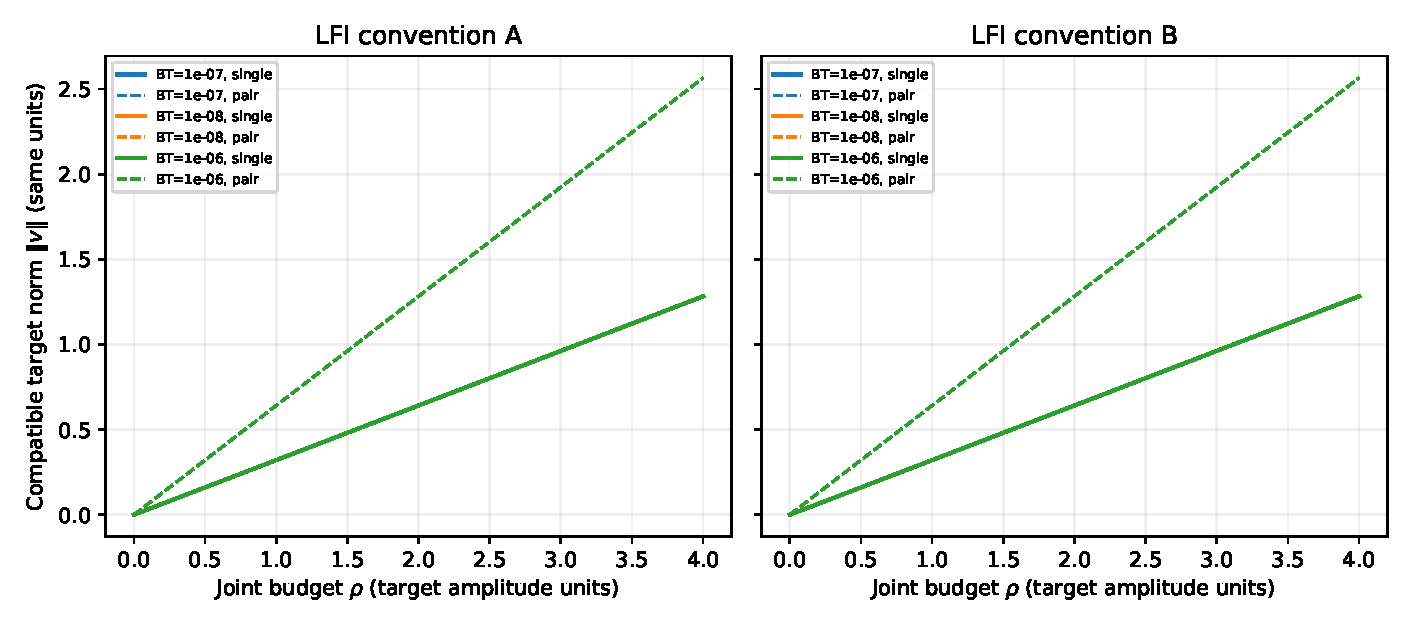
\includegraphics[width=.78\textwidth]{figures/common_frontier.pdf}
\caption{Attainable full-tensor displacement norm as a function of the declared joint moment budget $\rho$ under the same common metric in all six branches. Solid curves give the one-foreground limit $\rho/\ell_M$; dashed curves give the pairwise maximum $2\rho/\ell_M$. Colors distinguish the three HFI thresholds in each LFI panel. Nearly overlapping curves reflect the computed response-convention sensitivity. These are algebraic feasible-set frontiers for a free signed-moment class, not observed CMB amplitudes or confidence limits. Figure source: \texttt{consumer.py}, frozen R31 matrices.}
\label{fig:frontier}
\end{figure}

\begin{figure}[t]
\centering
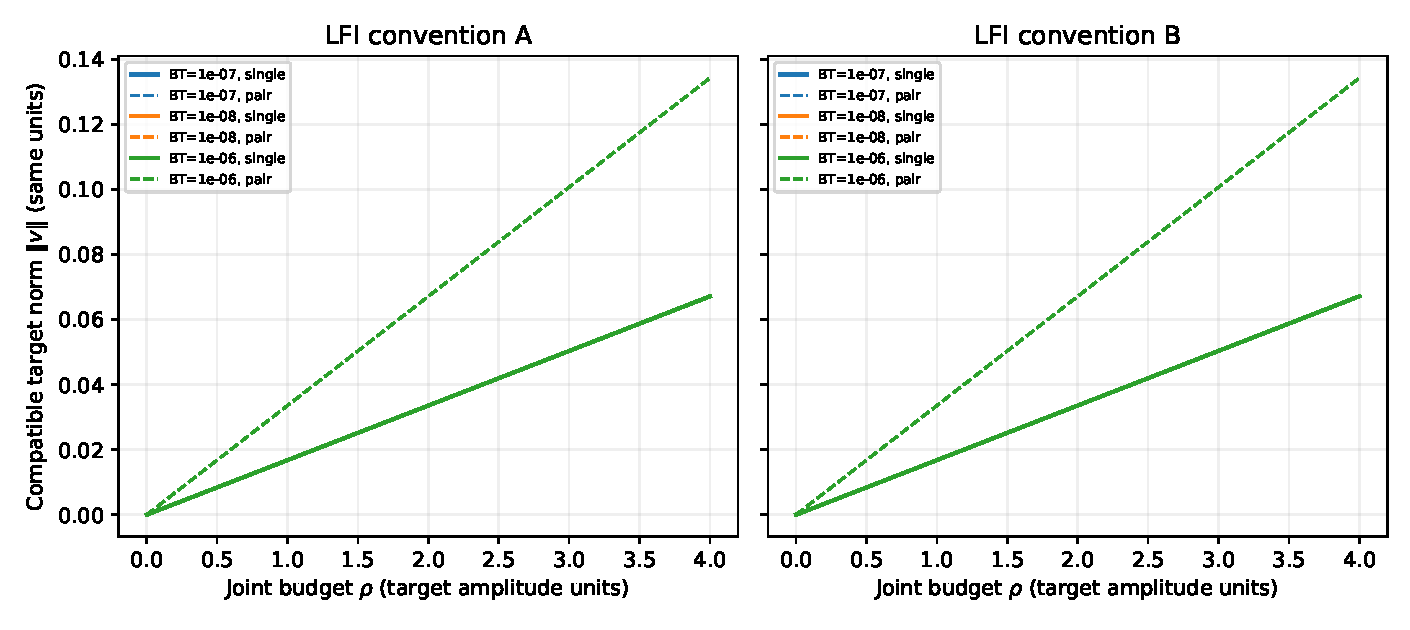
\includegraphics[width=.78\textwidth]{figures/raw_metric_sensitivity.pdf}
\caption{The same frontiers after explicitly replacing the common column-normalized metric with raw-coordinate $M=I_9$. Axis units and the factor-of-two distinction are unchanged; the shift in slope exposes the dependence on the bounded class. This panel is a metric-sensitivity calculation, not a second physical prior.}
\label{fig:raw}
\end{figure}

\section{Complete compatible target set and factor of two}

For specified $Y$, minimize the budget over $U$ at each proposed $s$. Applying Eq.~\eqref{eq:min} separately to the 24 columns gives
\begin{equation}
 U_s=M^{-1}F^{\mathsf T}K^{-1}(Y-a s^{\mathsf T}),\qquad
 J(s)=\operatorname{tr}\left[(Y-a s^{\mathsf T})^{\mathsf T}K^{-1}(Y-a s^{\mathsf T})\right].
 \label{eq:conditional}
\end{equation}
Define the full signed center and its irreducible cost by
\begin{equation}
 s_0=\frac{Y^{\mathsf T}K^{-1}a}{\ell_M^2},\qquad
 J_0=\operatorname{tr}\left[(Y-a s_0^{\mathsf T})^{\mathsf T}K^{-1}(Y-a s_0^{\mathsf T})\right]\ge0.
 \label{eq:center}
\end{equation}
Expanding $J(s)$ about $s_0$ makes the cross term vanish by the definition of $s_0$, so
\begin{equation}
 \boxed{\mathcal S_\rho(Y)=\{s\in\mathbb R^{24}:J_0+\ell_M^2\|s-s_0\|_2^2\le\rho^2\}.}
 \label{eq:set}
\end{equation}
It is empty for $\rho^2<J_0$, a singleton at exact equality, and otherwise a closed 24-dimensional ball centered at $s_0$ with radius $\sqrt{\rho^2-J_0}/\ell_M$. Its shape matrix in the given coordinate frame is $\ell_M^2 I_{24}$. We evaluate $J_0$ from a whitened residual equivalent to Eq.~\eqref{eq:center}, avoiding subtraction of nearly equal quadratic forms. Since the retained CMB response is exactly seven ones, exactly repeated finite rows of $Y$ have $s_0$ equal to their common row and $J_0=0$; at $\rho=0$ any exactly unequal rows give an empty set. Thus exact pure-target data give a singleton at zero budget and a full 24-dimensional ball of radius $\rho/\ell_M$ at positive budget. For other data, a homogeneous squared-amplitude error policy covers the factorization, triangular solves and projection; an unresolved boundary has status \texttt{BOUNDARY\_UNCERTAIN} or \texttt{NUMERIC\_BOUNDARY\_HOLD} and no asserted radius. This numerical policy is not a general interval certificate. Equation~\eqref{eq:set} is a deterministic compatible set, not a posterior or confidence region.

The zero-data illustration $Y=0$ has $s_0=0$ and $J_0=0$. One foreground can hide $v$ exactly when $\ell_M\|v\|\le\rho$, with $U=-c_Mv^{\mathsf T}$. For two foregrounds, each separately bounded by $\rho$, a common zero data table is obtained from
\begin{equation}
 s_1=v/2,\quad s_2=-v/2,\qquad
 U_1=-c_Mv^{\mathsf T}/2,\quad U_2=c_Mv^{\mathsf T}/2.
 \label{eq:pair}
\end{equation}
Each budget equals $\ell_M\|v\|/2$. Conversely $F(U_2-U_1)=a(s_1-s_2)$ and the triangle inequality give $\ell_M\|s_1-s_2\|\le\|U_2\|_M+\|U_1\|_M\le2\rho$. Thus the factor of two is both necessary and attained. At fixed generic $Y$, the diameter is $2\sqrt{\rho^2-J_0}/\ell_M$, when the set is nonempty. As $\rho\to\infty$ this finite obstruction disappears, consistently with the zero target quotient rank of the unrestricted nine-moment class. At $\rho=0$, $U=0$ and compatible data must be exactly $Y=a s^{\mathsf T}$.

\section{Numerical execution and scope}

The consumer checks the exact SHA-256 of the retained R31 result before reading any matrix. For each branch and metric, it solves $K$ by Cholesky, compares the minimum budget with an independently factored scaled SVD, checks $Fc_M=a$, the KKT equation, both null equations, metric normalization, nullspace orthogonality, the complete 24-coordinate null lift, and a positive norm increment. It exports each full $168\times24$ target operator $A$, $168\times216$ moment operator $B$, $216\times24$ compensator operator, $24\times168$ center map and $24\times24$ shape matrix. The synthetic controls act on all 24 basis vectors and a mixed signed vector, test boundary witnesses and 1\% beyond-boundary rejection, and construct a generic $Y$ with $J_0>0$ to test empty, constructed equality, and ball sectors. Targeted regressions repeat those cases after $10^{-6}$ and $10^6$ amplitude-unit conversions, check exact repeated and unequal rows, near-pure targets, center and radius scaling, and reject negative or nonfinite budgets. A bounded 80/120-digit calculation on the same cached matrices resolves cases that the binary64 error policy leaves undecided; its residual error is compared with the unchanged relative tolerance before a classification. Transporting the metric under nonzero column rescaling leaves $K$ and the set invariant; a fixed orthogonal carrier rotation preserves the budget and set. All controls are generated in the same execution as the reported table, with numerical residuals in Table~\ref{tab:checks}.

\begin{table}[t]
\caption{Smallest resolved singular value, relative $Fc=a$ residuals under both declared metrics, and largest relative full-tensor basis-action residual $\max_j\epsilon_j$ for the common-metric compensator. The residual gate is $10^{-10}$ for $Fc=a$ and $10^{-9}$ for the complete tensor actions.}
\label{tab:checks}
\centering\begin{tabular}{lrrrr}
\hline\hline
Branch & $\sigma_{\min}(FM^{-1/2})$ & $\|Fc_M-a\|/\|a\|$ & $\|Fc_I-a\|/\|a\|$ & $\max_j\epsilon_j$ \\
\hline
A\_BT\_1e-07 & 0.0055441 & 2.26e-14 & 1.13e-12 & 2.26e-14 \\
A\_BT\_1e-08 & 0.0055441 & 4.71e-14 & 7.16e-13 & 4.71e-14 \\
A\_BT\_1e-06 & 0.0055440 & 5.11e-14 & 1.22e-12 & 5.11e-14 \\
B\_BT\_1e-07 & 0.0055272 & 3.43e-14 & 2.17e-12 & 3.43e-14 \\
B\_BT\_1e-08 & 0.0055272 & 4.19e-14 & 1.61e-12 & 4.19e-14 \\
B\_BT\_1e-06 & 0.0055271 & 3.52e-14 & 1.03e-12 & 3.52e-14 \\
\hline\hline
\end{tabular}

\end{table}

The synthetic nonzero-data control has $J_0\simeq1.7174$ in the nominal branch. It realizes an empty set below $\sqrt{J_0}$ and radius $0.5$ at $\rho=\sqrt{J_0+\ell_M^2(0.5)^2}$. Its constructed equality case illustrates the exact singleton theorem; the computed boundary is labelled uncertain at finite precision. This is a numerical witness for Eq.~\eqref{eq:set}, not a sky realization. The smallest common-metric singular value and the complete basis residuals are shown in Table~\ref{tab:checks}; the exported binary64 coefficients, not only an internal intermediate, meet the residual gate.

The moment class permits signed independent harmonic and derivative coordinates. Physical component intensities, if positive, do not imply positivity of these harmonic or derivative coefficients. A physical version would need externally justified magnitude, coupling and truncation-remainder constraints, component-specific spatial responses, a real joint noise/calibration model, and a justified radius or prior. Those inputs are absent here. A nuisance with exactly the blackbody response remains confounded under this spectral model. We therefore make no statement about an observed quotient tensor, actual CMB amplitude, physical foreground filling fraction, calibrated exceedance, global tilt or Bianchi family. The retained status fields are $x=\mathrm{NOT\_MEASURED}$, $Q=\mathrm{NOT\_EVALUATED}$, $F_{\rm physical}=\mathrm{NOT\_EVALUABLE}$, $\Pi=\mathrm{NOT\_CALIBRATED}$, and $G_F=\mathrm{NOT\_APPLICABLE}$ because frequency is not depth. Complete source identities and claim ceilings are given in the accompanying \texttt{CLAIM\_SOURCE\_MAP.md}.

\end{document}
